Jacobson~\cite{j1989} first proposed to design succinct data structures.
He showed how to represent an ordinal trees on $n$ nodes using $2n+o(n)$ bits so
that computing the first child, the next sibling or the parent of any given node
takes $O(\lg n)$ time in the bit probe model.
Clark and Munro~\cite{cm1996} showed how to support the same operations in
constant time in the word RAM model with word size $\Theta(\lg n)$.
Since then, a lot of work has been done on succinct tree representations, to
support more navigational operations, to achieve compression, to provide support
for update operations, and so
on~\cite{mr1997,bdmr1999,grr2004,jss2007,ly2008,hms2012,fm2014,Navarro:2014:FFS:2620785.2601073}. 
Raman and Rao~\cite{rr2013} give a thorough survey of the state of the art.

In this paper, we present a parallel algorithm to construct the succinct tree
representation proposed recently by Navarro and
Sadakane~\cite{Navarro:2014:FFS:2620785.2601073}, referred to as
NS-representation throughout this paper.
This representation is the first to achieve a {\em redundancy}
of $O(n/\lg^c n)$ bits for any positive constant $c$.
The redundancy is the additional space used by the data structure above the
information-theoretic lower bound.
While all previous tree representations achieved a redundancy of $o(n)$ bits,
their redundancy was $\Omega(n \lg\lg n / \lg n)$ bits, that is, just slightly
sub-linear.
The NS-representation also supports a large number of
navigational operations in constant time (see Table~\ref{tbl:operations}); only
the work in \cite{hms2012,fm2014} supports two more operations.
The main reason we focus on this representation in this paper is an experimental
study on succinct trees~\cite{ACNSalenex10}, which showed that an implementation
of a simplified version ofthe NS-representation uses less space than other
existing representations in most cases and performs most operations faster.
Our goal in this paper is to alleviate the construction bottleneck of this
representation by exploiting multicore parallelism.

\begin{table}[t]
\begin{center}
\begin{tabular}{|>{\raggedright}p{2.4cm}|>{\raggedright\arraybackslash}p{5.2cm}|} \hline
\bf Operation                         & \bf Description        \\ \hline
$\child(x,i)$                         & Report $i$th child of node $x$\\
$\childrank(x)$                       & Report number of left siblings of node $x$\\
$\degree(x)$                          & Report degree of node $x$\\
$\depth(x)$                           & Report depth of node $x$\\
$\levelanc(x,i)$                      & Find ancestor of node $x$ that is $i $levels above node $x$ \\
$\subtreesize(x)$                     & Report number of nodes in the subtree rooted at node $x$ \\
$\height(x)$                          & Report height of the subtree rooted at $x$ \\
$\deepestnode(x)$                     & Find deepest node in the subtree rooted at node $x$\\
$\lca(x,y)$                           & Find lowest common ancestor of nodes $x$ and $y$ \\
$\lmostleaf(x)$ /$\rmostleaf(x)$      & Find leftmost/rightmost leaf of the subtree rooted at node $x$\\
$\leafrank(x)$                        & Report Number of leaves before node $x$ in preorder\\
$\leafselect(i)$                      & Find $i$th leaf from left to right\\
$\prerank(x)$ /$\postrank(x)$         & Report number of nodes preceding node $x$ in preorder/postorder\\
$\preselect$ /$\postselect(i)$        & Find $i$th node in preorder/postorder\\       
$\levellmost(i)$ /$\levelrmost(i)$    & Find leftmost/rightmost node among all the nodes at depth $i$ \\
$\levelsucc(x)$ /$\levelpred(x)$      & Find node immediately to the left/right of node $x$ among nodes at the same depth\\ \hline
$\access(i)$                          & Report the $i$th parenthesis $P[i]$        \\ 
$\findopen(i)$ /$\findclose(i)$       & Find the matching parenthesis of $P[i]$ \\
$\enclose(i)$                         & Find the closest enclosing matching parenthesis pair for $P[i]$ \\
$\rankopen(i)$ /$\rankclose(i)$       & Report the number of opening/closing parentheses in $P[1..i]$\\
$\selectopen(i)$ /$\selectclose(i)$   & Find the $i$th opening/closing parenthesis\\ \hline
\end{tabular}
\caption{Operations supported by the NS-representation, including operations
  on the corresponding balanced parenthesis sequence.}
\label{tbl:operations}
\end{center}
\end{table}

The NS-representation is based on the balanced parenthesis sequence $P$ of
the input tree, which is obtained by performing a preorder traversal
of the given tree and writing down an opening parenthesis when visiting
a node for the first time and a closing parenthesis after visiting
all its descendants.
Thus, the length of $P$ is $2n$.
The parenthesis sequence of the ordinal tree in Figure~\ref{figure:bp}, for
example, is $P = ((())((()())(()(())))()())$.

\begin{figure}
  \centering
  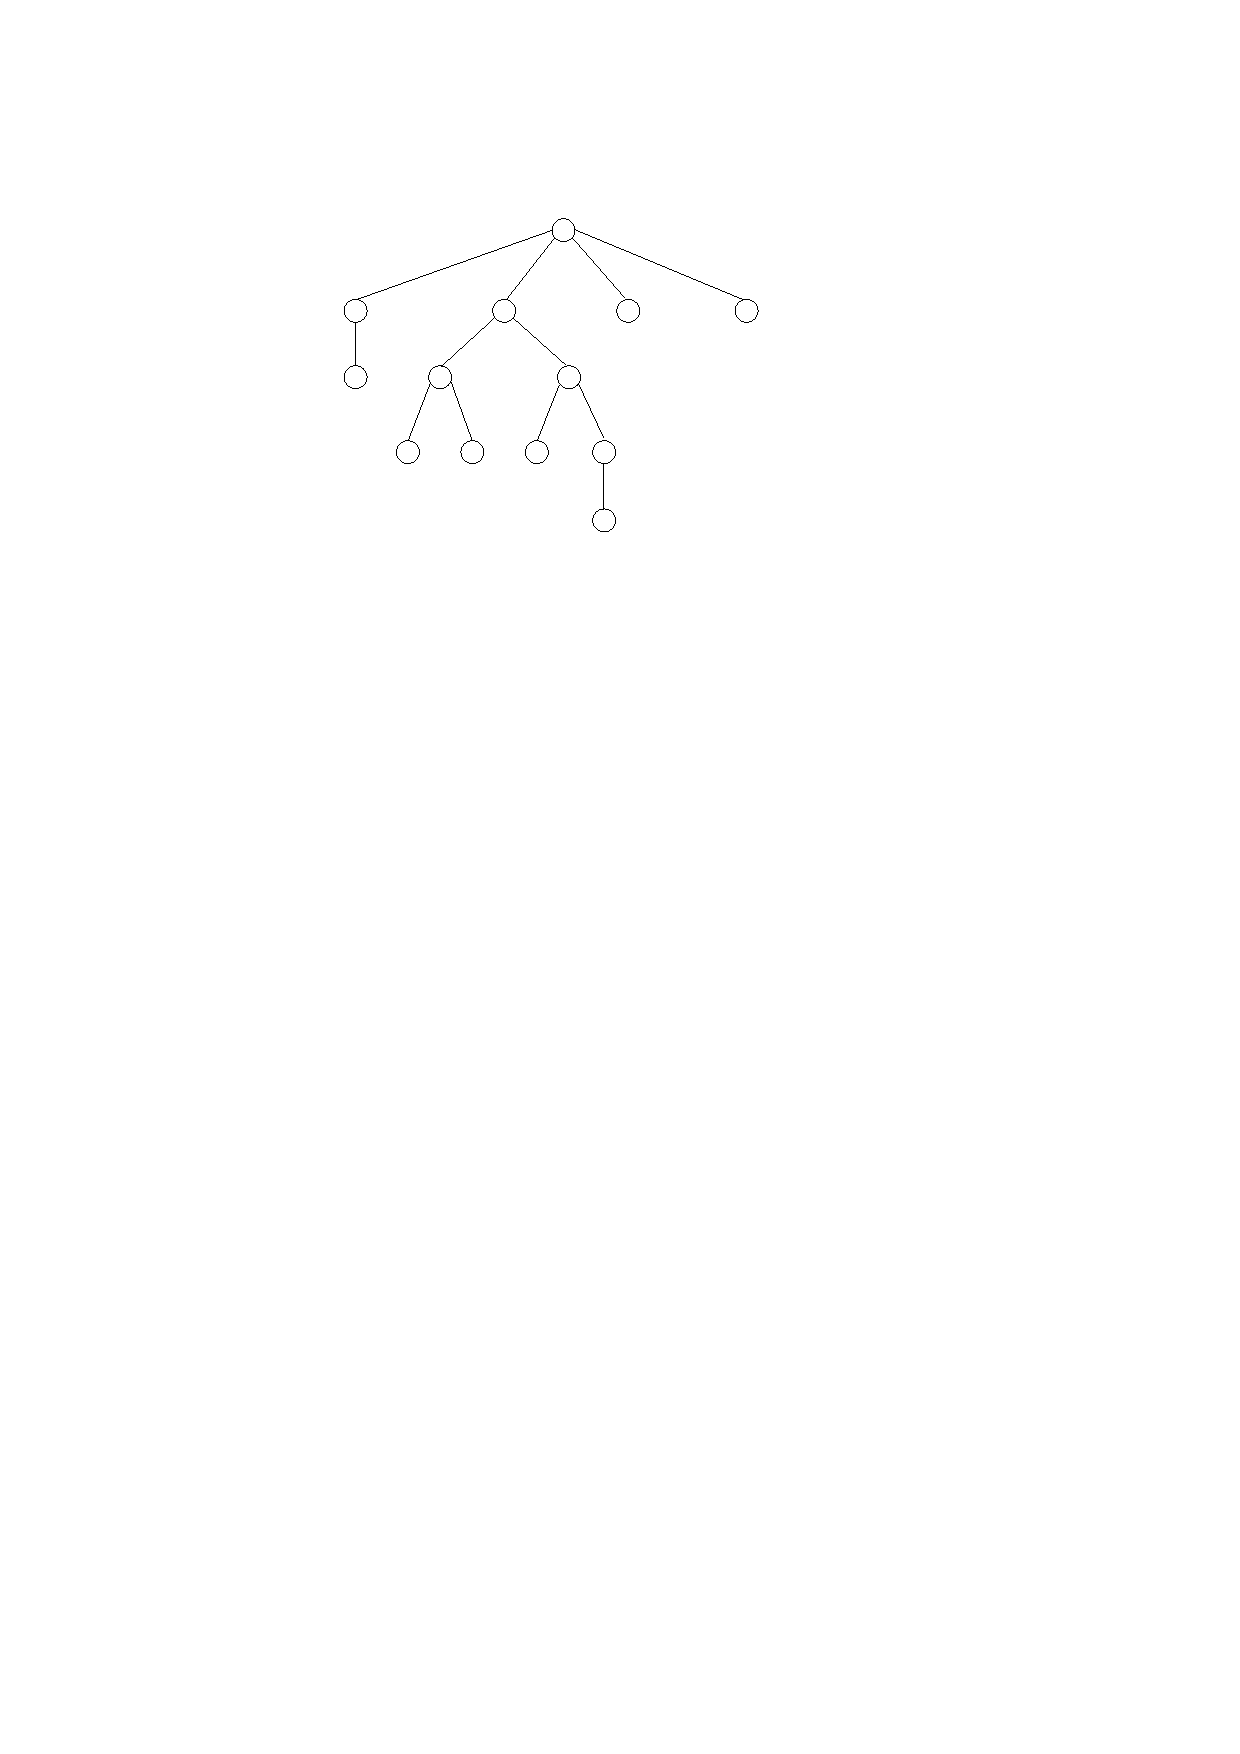
\includegraphics[scale=0.5]{images/bp.pdf}
  \caption{An ordinal tree used as an example.}
  \label{figure:bp}
\end{figure}

The NS-representation is not the first structure to use balanced parentheses to
represent trees.
Munro and Raman~\cite{mr1997} were the first to design succinct representations
of balanced parentheses and used them to represent ordinal trees succinctly by
reducing a set of navigational operations on trees to operations on their
balanced parenthesis sequences.
Their solution supports only a subset of the operations listed in
Table~\ref{tbl:operations}.
Additional operations can be supported using  auxiliary data
structures~\cite{ly2008}.
To support all operations in Table~\ref{tbl:operations}, many auxiliary data
structures are required, which add to the size of the final data structure
and make it complex in both theory and practice.
The main novelty of Navarro and Sadakane's
work~\cite{Navarro:2014:FFS:2620785.2601073} lies in the strategy they used to
reduce a large set of operations on trees and balanced parenthesis sequences to
a small set of \emph{primitive operations}.
Representing $P$ as a bit vector storing a $1$ for each opening parenthesis
and a $0$ for each closing parenthesis, these primitive operations are the
following.
Here, $g$ is an arbitrary function on $\{0,1\}$.
\begin{align*}
\sumop(P,g,i,j) &= \textstyle\sum_{k=i}^jg(P[k])\\
\fwdsearch(P,g,i,d) &= \min\{j \mid j \ge i, \sumop(P,g,i,j) = d\}\\
\bwdsearch(P,g,i,d) &= \max\{j \mid j \le i, \sumop(P,g,j,i) = d\}\\
\rmq(P,g,i,j) &= \min\{\sumop(P,g,i,k) \mid i\le k\le j\}\\
\RMQ(P,g,i,j) &= \max\{\sumop(P,g,i,k) \mid i\le k\le j\}\\
\rmqi(P,g,i,j) &= \argmin_{k\in[i,j]}\{\sumop(P,g,i,k)\}\\
\RMQi(P,g,i,j) &= \argmax_{k\in[i,j]}\{\sumop(P,g,i,k)\}
\end{align*}
Navarro and Sadakane defined three functions on $[0,1]$:
\begin{align*}
  \pi  &: 1 \mapsto 1\quad 0 \mapsto -1\\
  \phi &: 1 \mapsto 1\quad 0 \mapsto 0\\
  \psi &: 1 \mapsto 0\quad 0 \mapsto 1
\end{align*}
Most of the operations in Table~\ref{tbl:operations} can then be supported using
the primitive operations by setting $g$ to be $\pi$, $\phi$ or~$\psi$.
For example, $\findclose(i) = \fwdsearch(P,\pi,i,0)$.
Thus, it suffices to support the operations in Table~\ref{tbl:operations} for
$g = \pi$, $g = \phi$ or $g = \psi$, as well as a few navigational operations
that cannot expressed using these primitive operations, which are $\degree$,
$\child$, $\childrank$ and the four operations in Table~\ref{tbl:operations}
related to leaf nodes.
To support the primitive operations, Navarro and Sadakane designed a simple data
structure called \emph{Range Min-Max Tree} ({\tt RMMT}) (see next subsection).
It supports the primitive operations in logarithmic time when used to represent
the entire sequence~$P$.
To achieve constant-time operations, $P$ is further partitioned into chunks.
Each chunk is represented using a {\tt RMMT}, which can support primitive
operations inside the chunk in constant time if the chunk is small enough.
Additional data structures are used to support operations on the entire sequence
$P$ in constant time.

\subsubsection{The Range Min-Max Tree}

Let $w$ denote the number of bits in a word.
The range min-max tree ({\tt RMMT}) is designed to support the primitive
operations for functions $\pi$, $\phi$, and $\psi$.
We first describe how to construct a {\tt RMMT} for the function $\pi$ and
later show how it can be easily augmented to support the primitive operations
for the other two functions.
Recall that $T$ denotes the input tree on $n$ nodes, and $P$ represents its
balanced parenthesis sequence, where $P[i] = 1$ iff the $i$th
parenthesis is an opening parenthesis.
To define the {\tt RMMT}, we partition $P[1..2n]$ into disjoint chunks of
a size $s \le w/2$ to be chosen later.
For simplicity, we assume that the length of $P$ is a multiple of~$s$.
The {\tt RMMT} is a complete $k$-ary tree over the sequence of these chunks,
for some \emph{arity} $k \ge 2$ to be chosen later (see
Figure~\ref{fig:RangeMinMaxTree}).

Next define the following five arrays $E$, $e$, $m$, $M$, and $n^*$.
These arrays are only used in the description and are not stored explicitly
in the data structure.
The {\em excess} at position $i$ of $P$ is defined as $\sumop(P,\pi,0,i) =
\sum_{k=0}^{i} \pi(P[k])$.
$E$ has length $2n$ and $E[i]$ is the excess at position $i$.
The other four arrays are of length $2n/s$ each.
$e[i]$ stores the excess at position $is$, that is, at the end of the $i$th
chunk.
$m[i]$ and $M[i]$ store the minimum and maximum excess at any position in the
$i$th chunk, respectively.
$n^*[i]$ stores the number of positions in the $i$th chunk that have the
minimum excess value $m[i]$.
Each internal node, $u$, of the {\tt RMMT} also stores four similar values
$e[u]$, $m[u]$, $M[u]$, and $n^*[u]$, which have the same meaning as defined
above with respect to the subsequence of $P$ that is the concatenation of the
chunks corresponding to descendant leaves of $u$.
These values are illustrated in Figure~\ref{fig:RangeMinMaxTree}.
As the {\tt RMMT} is a complete tree, we do not store its structure explicitly.
Instead, we can simply store the values associated with its nodes in four arrays
$e'$, $m'$, $M'$, and $n'$ indexed like a $k$-ary heap.

\begin{figure}[t]
  \centering
  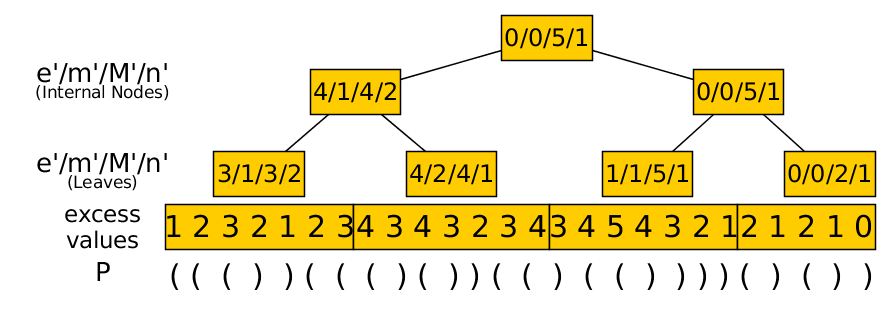
\includegraphics[scale=0.18]{./images/Range-min-max-tree.png}
  \caption{Range min-max tree}
  \label{fig:RangeMinMaxTree}
\end{figure}

Combined with a standard succinct data structure technique called {\em table
  lookup}, a {\tt RMMT} can support the primitive operations for $\pi$, as well
as $\degree$, $\child$ and $\childrank$ queries.
For example, consider $\fwdsearch(P,\pi,i,d)$.
We first check the chunk containing $P[i]$ to see if the answer is inside the
same chunk.
This can be done in constant time by constructing a universal lookup table whose
content does not depend on $P$: For each possible bit vector of length $s$,
and each of the $s$ position in the bit vector, we store the answer of
$\fwdsearch(P,\pi,i,d)$ if it can be found inside this bit vector, or $-1$
otherwise.
As there are $2^s$ bit vectors of length $s$, this table uses
$2^s\poly(s)$ bits.
If we find the  answer by performing a table lookup for the chunk containing
$P[i]$, then we return.
Otherwise, we search among the $m$ and $M$ values of the right siblings of the
leaf node $u$ corresponding to this chunk, to find the closest right sibling
that contains the answer if the answer is within chunks represented by these
siblings.
If the $m$ and $M$ values of the $k$ children of each internal node can be
packed into $O(w)$ bits, i.e., $k \lg n = O(w)$, then we can again construct
universal lookup tables for internal nodes to perform this step in constant
time.
We repeat this process until we find a right sibling, $v$, of an ancestor of $u$
whose corresponding substring of $P$ contains the answer.
We then use a similar idea to descend down the tree starting from $v$ to look
for the leaf descendant of $v$ containing the result.
Thus, we can support $\fwdsearch$ in $O(h)$ time, where $h$ is the height of the
{\tt RMMT}, provided that $k \lg n = O(w)$.

To support the primitive operations for functions $\phi$ and~$\psi$, we can
define six arrays $e'_{\phi}$, $m'_{\phi}$, $M'_{\phi}$, $e'_{\psi}$,
$m'_{\psi}$ and $M'_{\psi}$ which are similar to $e'$, $m'$ and $M'$ defined for
$\pi$ ($n'$ is defined to support $\degree$, $\child$ and $\childrank$ only, so
we need not define similar arrays for $\phi$ and $\psi$).
We make use of the following three observations to avoid storing these six
arrays explicitly: $\sumop(P, \phi, 0, i)$ and $\sumop(P, \psi, 0, i)$ are
nondecreasing, $\sumop(P, \phi, 0, i) + \sumop(P, \psi, 0, i) = i$ and
$\sumop(P, \phi, 0, i) - \sumop(P, \psi, 0, i) = \sumop(P, \pi, 0, i)$.
Thus, the each value in these six arrays can be computed in constant time
without storing them explicitly.
We only need to store the universal tables needed to support primitive
operations for $\phi$ and $\psi$.

To support $\leafrank$, $\leafselect$, $\lmostleaf$ and\break $\rmostleaf$, we
define a conceptual bit vector $P_1[1..2n]$ in which $P_1[i] = 1$ iff $P[i] = 1$
and $P[i+1] = 0$.
Hence each $1$-bit in $P_1$ corresponds to a leaf node.
The above operations then reduce to $\rankop$ and $\selop$ operations on
$P_1$, where $\rankop(P_1, i)$ returns the number of $1$s in $P_1[1..i]$ and
$\selop(P_1, i)$ returns the position of the $i$th $1$-bit in $P_1$.
For example, we have $\leafrank = \rankop(P_1, i)$.
$\rankop$ and $\selop$ operations can be further reduced to $\sumop$ and
$\fwdsearch$ for the function $\phi$ on $P_1$, which can be supported using
another range min-max tree.
Since any $O(w)$ bits in the sequence $P_1$ can be computed from $P$ in constant
time using table lookup, $P_1$ itself need not be stored explicitly, while the
cost of storing the information for the internal nodes of this range min-max
tree is dominated by the space usage of the range min-max tree for $P$.

To analyze the space usage of the entire data structure, we observe that if we
store $P$, $e'$, $m'$, $M'$ and $n'$ explicitly in a straightforward manner, the
space usage  would be $2n + \frac{k}{k-1} \cdot \frac{n}{s} \cdot \lg n$.
Navarro and Sadakane commented that choosing $s = w/2$ and $k = w / \lg n$ gives
a simple structure supporting all the operations in Table~\ref{tbl:operations}
in $O(\lg n)$ time.
However, if the trees are large enough that $w = \Theta(\lg n)$, then $e'$,
$m'$, $M'$ and $n'$ would occupy $O(n)$ bits, and the size of the representation
would be greater than is typical for a succinct tree representation,
which would use $2n+o(n)$ bits.
To reduce the overall space cost to $2n+o(n)$ bits, we can set
$s = \lceil w\lg n\rceil$ and $k = 2$.
With these parameters, looking for a potential answer to a query within a chunk
requires $O(\lg n)$ table lookups, which is dominated by the $O(\lg n)$ cost of
traversing the tree to answer queries.
Thus, the overall query cost remains $O(\lg n)$.
Moreover, for $k = 2$, universal tables are not needed for internal nodes.
Thus, we have the following lemma:

\begin{lemma}\label{lem:lg}
  An ordinal tree and its balanced parentheses sequence can be represented using
  range min-max trees in $2n + o(n)$ bits, where $n$ is the number of nodes in
  the tree.
  This structure supports all operations in Table~\ref{tbl:operations} in
  $O(\lg n)$ time.
\end{lemma}

Navarro and Sadakane showed how to use the structure described so far as a
building block for a more complicated structure that supports all operations in
Table~\ref{tbl:operations} in constant time.
Due to its complexity, however, this structure is much more difficult to
implement and may not be efficient in practice.
On the other hand, the structure described here has been experimentally verified
to be very small and achieve very good query performance in
practice~\cite{ACNSalenex10}.
This is the reason we chose this structure as the basis for our work presented
in this paper.
